\section[Automatisation]{Automatisation du cycle de vie d'une application}

\subsection{Définition}
\begin{frame}{\subsecname}
	\begin{block}{Selon le Larousse}
		\frquote{Exécution totale ou partielle de tâches techniques par des machines fonctionnant sans intervention humaine.}
	\end{block}
\end{frame}

\subsection{Pourquoi ?}
\begin{frame}{\subsecname}
	\begin{center}
		\begin{minipage}{0.5\textwidth}
			\begin{itemize}
				\item Besoin de factorisation -- harmonisation
				\note[item]{Besoin d'harmonisation, besoins communs entre portail (mail) et mises à jour de ces derniers compliqués.}
				\pause
				\item Faciliter les tests
				\note[item]{Tests auto, on en reparle après}
				\pause
				\item Pas de réel environnement de test
				\note[item]{Staging qui n'était pas déployé automatiquement et pas forcément à jour.}
			\end{itemize}
		\end{minipage}
	\end{center}
\end{frame}

\subsection{Tests}
\begin{frame}{\subsecname}
\begin{block}{Mise en place}
	\begin{itemize}
		\item Preuve de concept des tests Drupal
		\item Écriture de \frquote{modèles de tests} pour encourager la pratique
		\item Build qualité -- test de mise à jour
	\end{itemize}
\end{block}
\end{frame}

\subsection{Gestion de projet}
\begin{frame}{KPI}
	\begin{columns}[onlytextwidth]
		\column{.4\textwidth}
		\begin{block}{}
			\begin{itemize}
				\item Temps de déploiement réduit (\textasciitilde30min $\rightarrow$ 5min)
				\note[item]{Avant : construction package de livraison à la main, upload, potentielle erreur de droits... Du temps gagné, donc de l'argent }
				\pause
				\item Livrer plus rapidement de la valeur métier
				\note[item]{Réduire délai entre poste développeur -- test -- recette -- preprod -- prod et passer plus de temps sur de la valeur métier que de la livraison}
			\end{itemize}
		\end{block}
		\column{.5\textwidth}
		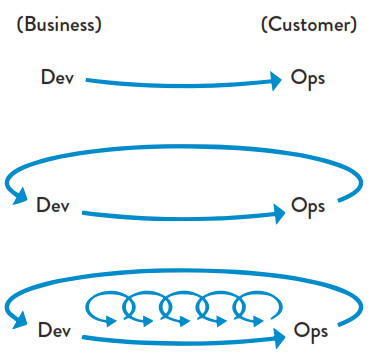
\includegraphics[width=0.8\linewidth]{img/devops-objective.jpg}
	\end{columns}
	\note[item]{KPI vracs : Rentabilité financière, car tâches prennent moins de temps, réduction time to market}
\end{frame}

%\begin{frame}{Work In Progress}
%	\begin{block}{Objectif : le réduire}
%	\end{block}
%	\note[item]{JIRA pour s'organiser dans les tâches. Permet de voir que si quelqu'un sur plusieurs sujet, cest qu'il y a un soucis et qu'il y a un potentiel blocage}
%	\centering \movie[width=8cm,height=5cm]{}{img/wip.gif}
%\end{frame}

\begin{frame}{Code review}
	\centering 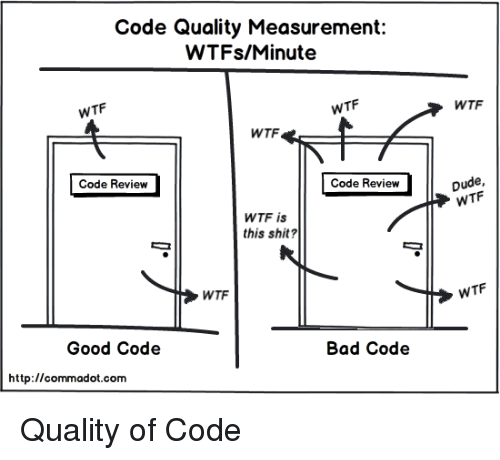
\includegraphics[width=0.50\textwidth]{img/code-review.png}
	\note[item]{Entraine une plus grande communication au sein de l'équipe, et une résilience de l'information même s'il peut y avoir des différents comme l'illustre l'image ci-contre}
\end{frame}

\subsection[Développement]{Pratiques de développement}

\begin{frame}{Environnement de développement local}
	\begin{overprint}
		\onslide<1> 
		\begin{block}{Installation d'un portail localement -- Avant}
			\note[item]{README trop long, pas maintenu, pas assez détaillé, qui se contredise, différentes selon les portails, doc PAS A JOUR}
			\begin{columns}[onlytextwidth]
				\column{.4\textwidth}
				\begin{itemize}
					\item Chaque portail différent
					\item \textasciitilde 10 étapes
					\item 20 minutes $\longleftrightarrow$ 2 heures
				\end{itemize}
				\column{.5\textwidth}
				\movie[width=6cm,height=6cm]{}{img/no-please-no.gif}
			\end{columns}
		\end{block}
		\onslide<2> 
		\begin{block}{Installation d'un portail localement -- Maintenant}
			\note[item]{Même procédure d'installation pour tous les portails. Garanti reproductiblité en définissant les modules actifs ainsi que certaines configurations communes. Passage de Xh à 10min, temps de téléchargement des dépendances compris. Pile le temps de prendre un café !}
			\begin{columns}[onlytextwidth]
				\column{.4\textwidth}
				\begin{itemize}
					\item Identique pour tous les portails
					\item 5 commandes
					\item 10 minutes
				\end{itemize}
				\column{.3\textwidth}
				\movie[width=4cm,height=4cm]{}{img/coffee.gif}
			\end{columns}
		\end{block}
	\end{overprint}
\end{frame}

\subsection{Conduite de changement}
\begin{frame}{\subsecname}
	\begin{columns}[onlytextwidth]
		\column{.4\textwidth}
		\begin{itemize}
			\item Phase de réflexion commune
			\note[item]{travail \& validation par plusieurs architectes applicatifs}
			\item Accompagnement
			\note[item]{pour les migrations/ changement d'habitude}
			\item Dépréciation ancienne structure de code sur 3 mois
			\note[item]{garantir que il n'y aura pas de perte de code ni d'historique lors de la transition}
		\end{itemize}
		\column{.6\textwidth}
		\begin{figure}
			
\includegraphics[width=0.6\linewidth]{img/rome.jpg}
			\captionsetup{labelformat=empty}
			\caption{https://twitter.com/drzarrow/status/479245604552704000}
			\label{fig:rome}
		\end{figure}
	\end{columns}
\end{frame}
